\documentclass[letterpaper]{article}
\usepackage[utf8]{inputenc}
\usepackage[spanish, mexico]{babel}
\usepackage{amssymb, amsmath}
\usepackage{stackengine}
\usepackage{graphicx}
\usepackage{ mathrsfs }
\usepackage{lipsum}
\usepackage{dsfont}
\usepackage[margin=1.5cm,
vmargin={1.5cm,0.7cm},
includefoot]{geometry}
\usepackage{setspace}
\usepackage{subcaption}
\usepackage{tocloft}
\usepackage{upgreek}
\usepackage{amsthm}
\usepackage{graphicx}
\usepackage{paralist}
\usepackage{fancyhdr}
\usepackage{lmodern}
\usepackage{tcolorbox}
\usepackage{color}
\usepackage{tikz}
\usepackage{wasysym}
\usepackage{textgreek, marvosym}
\tcbuselibrary{skins,breakable}
\pagestyle{fancy}

\renewcommand{\headrulewidth}{0.4pt}
\renewcommand{\footrulewidth}{0.4pt}

\renewcommand{\d}{\partial}

\providecommand{\abs}[1]{\left|#1\right|}
\providecommand{\norm}[1]{\left|\left|#1\right|\right|}														  
\providecommand{\pint}[1]{\langle#1\rangle}														  
\newcommand{\V}{\mathds{V}}

\newcommand{\W}{\mathds{W}}

\newcommand{\F}{\mathds{F}}

\newcommand{\tq}{ \quad \cdot  \backepsilon \cdot \quad }

\newcommand{\ld}{\lim\limits_{x \to 0^{+}}}

\newcommand{\li}{\lim\limits_{x \to 0^{-}}}

\newcommand{\la}{\lim\limits_{x \to a}}

\renewcommand{\l}{\ell}

\newcommand{\R}{\mathds{R}}

\newcommand{\Po}{\mathds{P}_2(\mathds{R})}

\renewcommand{\*}{\cdot}

\makeatletter
\renewcommand*\env@matrix[1][\arraystretch]{%
	\edef\arraystretch{#1}%
	\hskip -\arraycolsep
	\let\@ifnextchar\new@ifnextchar
	\array{*\c@MaxMatrixCols c}}
\makeatother

\newtheorem{theorem}{Teorema}[]
\theoremstyle{definition}
\newtheorem{definition}{Definición}


\begin{document}
	
	\setlength{\unitlength}{1cm}
	\thispagestyle{empty}
	\begin{picture}(19,3)
	\put(-0.5,1.2){
\includegraphics[scale=.20]{img/unam1.png}}
	\put(16,1){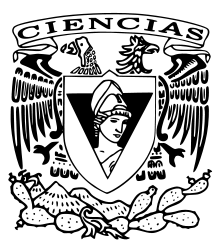
\includegraphics[scale=.29]{img/fciencias1.png}}
	\end{picture}
	
	\begin{center}
		\vspace{-114pt}
		\textbf{\large Matemáticas para las Ciencias II}\\
		\textbf{ Semestre 2020-2}\\
		Prof. Pedro Porras Flores\\
		Ayud. Irving Hernández Rosas \\
		\textbf{Tarea Examen II}\\[0.15cm]
		Kevin Ariel Merino Peña\footnote{Número de cuenta 317031326}\\ [0.12cm]
		\today
	\end{center}
	\vspace{-10pt}
	\rule{19cm}{0.3mm}
	
\noindent Realice los siguientes ejercicios, escribiendo el procedimiento claramente. Y recuerden la tarea-examen se entregan de manera individual.\\

\noindent1. El volumen específico $ V $, la presión $ P $  la temperatura $ T $ de un gas van der Waals están relacionados por
\[ P = \dfrac{RT}{V - \beta} - \dfrac{\alpha}{V^2} \] donde $ \alpha, \beta $ y $ R $ son constantes.\\

a) Encuentre $ \dfrac{\d T}{\d P}, \dfrac{\d P}{\d V} $ y $ \dfrac{\d V}{\d T} $.\\

Identifique qué variables son constantes e interprete físicamente cada derivada parcial.\\

b) Verifique $ \left( \dfrac{\d T}{\d P}\right) \left( \dfrac{\d P}{\d V}\right)\left( \dfrac{\d V}{\d T}\right) = -1 $\\

\noindent2. Considere una función de temperatura $ T(x,y) = x\sin(y) $ Trazar algunas curvas de nivel. Calcula $ \nabla T $ y explique su significado.\\

\noindent3. Encuentre el plano tangente a la superficie $ z = x^2 + y^2 $ en el punto $ (1,-2,5) $. Explica el significado geométrico para esta superficie del gradiente de $ f(x,y)= x^2 + y^2 $\\

\noindent4. Un bicho se encuentra en un entorno tóxico. El nivel de toxicidad está dado por $ T(x,y) = 2x^2 - 4y^2 $. Si el bicho está en $ (-1,2) $. ¿En qué dirección debería moverse para reducir la toxicidad más rápido.\\

\noindent5. El desplazamiento en el tiempo $ t $ y la posición horizontal en la recta $ x $ de una cierta cuerda de violín, está dada por $$ u(x,t) = \sin(x - 6t) + \sin(x+6t) $$ Calcule la velocidad de la cuerda en $ x = 1 $ cuando $ t = \dfrac{1}{3} $.\\

\noindent6. La altura $ h $ del volcán hawaiano Mauna Loa se describe (aproximadamente) por la función $$ H(x,y) = 2.59 - 0.00024y^2 - 0.00065x^2 $$donde $ h $ es la altura sobre el nivel del mar en millas y $ x $ e $ y $ se miden de \textbf{este} a \textbf{oeste} y de \textbf{norte} a \textbf{sur}, también en millas desde la cima de la montaña. En $ (x,y) = (-2,-4) $:\\

a) ¿Qué tan rápido amenta la altura en la dirección $ (1,1) $(es decir, hacia el noreste)? Exprese su respuesta en millas de altura por milla de distancia horizontal recorrida.\\

b) ¿En qué dirección es el camino ascendente más empinado?

\end{document}